%% W2 -- AICS @ AAAI-27 -- final paper source, taken verbatim from Overleaf (the source of truth for all text).
%% Not generated: edit in Overleaf and copy the main .tex here. Tables 2, 3, 5 are inlined; paper/tables/ holds
%% the same tables as generated by scripts/revision/final.py. Compile with aaai2027.sty and aaai2027.bst from the
%% AAAI-27 author kit, references.bib and fig_method.pdf.
\documentclass[letterpaper]{article} % DO NOT CHANGE THIS
\usepackage{aaai2027}  % DO NOT CHANGE THIS
% The serif, sans-serif, and monospaced fonts are loaded automatically by
% aaai2027.sty (newtxtext, helvet, courier). DO NOT add \usepackage{times},
% \usepackage{helvet}, \usepackage{courier}, or any other font package.
\usepackage[hyphens]{url}  % DO NOT CHANGE THIS
\usepackage{graphicx} % DO NOT CHANGE THIS
\urlstyle{rm} % DO NOT CHANGE THIS
\def\UrlFont{\rm}  % DO NOT CHANGE THIS
\usepackage{natbib}  % DO NOT CHANGE THIS AND DO NOT ADD ANY OPTIONS TO IT
\usepackage{caption} % DO NOT CHANGE THIS AND DO NOT ADD ANY OPTIONS TO IT
\frenchspacing  % DO NOT CHANGE THIS
%
% These are recommended to typeset algorithms but not required. See the subsubsection on algorithms. Remove them if you don't have algorithms in your paper.
\usepackage{algorithm}
\usepackage{algorithmic}

%
% These are recommended to typeset listings but not required. See the subsubsection on listing. Remove this block if you don't have listings in your paper.
\usepackage{newfloat}
\usepackage{listings}
\DeclareCaptionStyle{ruled}{labelfont=normalfont,labelsep=colon,strut=off} % DO NOT CHANGE THIS
\lstset{%
	basicstyle={\footnotesize\ttfamily},% footnotesize acceptable for monospace
	numbers=left,numberstyle=\footnotesize,xleftmargin=2em,% show line numbers, remove this entire line if you don't want the numbers.
	aboveskip=0pt,belowskip=0pt,%
	showstringspaces=false,tabsize=2,breaklines=true}
\floatstyle{ruled}
\newfloat{listing}{tb}{lst}{}
\floatname{listing}{Listing}

%
% Recommended for better-looking tables
\usepackage{booktabs}

%
% Keep the \pdfinfo as shown here. There's no need
% for you to add the /Title and /Author tags.
\pdfinfo{
/TemplateVersion (2027.2)
}

% DISALLOWED PACKAGES
% \usepackage{authblk} -- This package is specifically forbidden
% \usepackage{balance} -- This package is specifically forbidden
% \usepackage{CJK} -- This package is specifically forbidden
% \usepackage{float} -- This package is specifically forbidden
% \usepackage{flushend} -- This package is specifically forbidden
% \usepackage{fullpage} -- This package is specifically forbidden
% \usepackage{geometry} -- This package is specifically forbidden
% \usepackage{hyperref} -- This package is specifically forbidden
% \usepackage{navigator} -- This package is specifically forbidden
% (or any other package that embeds links such as navigator or hyperref)
% \usepackage{indentfirst} -- This package is specifically forbidden
% \usepackage{layout} -- This package is specifically forbidden
% \usepackage{multicol} -- This package is specifically forbidden
% \usepackage{nameref} -- This package is specifically forbidden
% \usepackage{savetrees} -- This package is specifically forbidden
% \usepackage{setspace} -- This package is specifically forbidden
% \usepackage{stfloats} -- This package is specifically forbidden
% \usepackage{tabu} -- This package is specifically forbidden
% \usepackage{titlesec} -- This package is specifically forbidden
% \usepackage{tocbibind} -- This package is specifically forbidden
% \usepackage{ulem} -- This package is specifically forbidden
% \usepackage{wrapfig} -- This package is specifically forbidden
% DISALLOWED COMMANDS
% \nocopyright -- Your paper will not be published if you use this command
% \addtolength -- This command may not be used
% \balance -- This command may not be used
% \baselinestretch -- Your paper will not be published if you use this command
% \clearpage -- No page breaks of any kind may be used for the final version of your paper
% \columnsep -- This command may not be used
% \newpage -- No page breaks of any kind may be used for the final version of your paper
% \pagebreak -- No page breaks of any kind may be used for the final version of your paper
% \pagestyle -- This command may not be used
% \tiny -- This is not an acceptable font size.
% \vspace{- -- No negative value may be used in proximity of a caption, figure, table, section, subsection, subsubsection, or reference
% \vskip{- -- No negative value may be used to alter spacing above or below a caption, figure, table, section, subsection, subsubsection, or reference

\setcounter{secnumdepth}{0} %May be changed to 1 or 2 if section numbers are desired.

% ---- paper-specific packages and macros (from the draft) ----
\usepackage{amsmath,amssymb}
\usepackage{xcolor}
\setlength{\emergencystretch}{3em}
\newcommand{\todo}[1]{\textbf{[TODO: #1]}}
\newcommand{\vf}{\textsuperscript{\dag}}
\newcommand{\x}[1]{\,(#1)}
\newcommand{\ci}[2]{{\scriptsize[$#1$, $#2$]}}
\newcommand{\bk}{\textsuperscript{*}}
\newif\ifflags
\ifdefined\showflags \flagstrue \else \flagsfalse \fi
\newcommand{\flag}[1]{\ifflags\textcolor{red}{\textsuperscript{\textbf{[#1]}}}\fi}

\title{Can LLMs Compile Cyber Threat Intelligence into Adversary Behavior Models? Evaluating Predictive Value and Quotation Fidelity}
\author{
    Jack Moody\textsuperscript{\rm 1},
    Iain Cruickshank\textsuperscript{\rm 2}
}
\affiliations{
    \textsuperscript{\rm 1}Johns Hopkins University, Baltimore, MD, USA\\
    \textsuperscript{\rm 2}Carnegie Mellon University, Pittsburgh, PA, USA\\
    jmoody11@jhu.edu, icruicks@andrew.cmu.edu
}

\begin{document}
\maketitle

\begin{abstract}
We evaluate whether language models can compile cyber threat intelligence (CTI) reports into predictive models of adversary behavior. From 23 reports on four actors, we extract ATT\&CK tactic relations and aggregate report-level support into smoothed first-order transition kernels. We compare two frontier and three local models against public emulation plans, excluding plan-cited sources from the input corpus. Frontier-model kernels outperform the tested ATT\&CK frequency baseline and achieve approximately two to six times the edge precision of size-matched random predictions. Their mean information gain over uniform is positive on all four plans, although several uncertainty intervals include zero. Actor-name-only controls show that report benefit depends on actor and metric. For menuPass, no-report outputs have higher edge-F1 and precision enrichment without an established likelihood advantage. Each of two 14B open-weight models reaches at least 80\% of Claude Opus's edge-F1 on three of four actors (not the same three), but 7--30\% of their evidence quotations fail source matching, compared with at most 0.5\% for the frontier models. We express information gain as the average likelihood-ratio score change relative to a uniform actor prior and derive an upper bound on positive score change. Two case studies on recorded emulation and red-team executions do not establish robust actor-specific detection gains. We provide a checklist for assessing the predictive value, quotation fidelity, and detection utility of LLM-compiled CTI.
\end{abstract}

\section{Introduction}

Cyber threat intelligence (CTI) is central to the work of a security operations center (SOC). Threat hunters rely on it to learn how adversaries operate: their tactics, techniques, and procedures (TTPs), their tools, and their patterns of life. CTI is written as narrative prose for people, and a good report tells an intrusion in order: how the actor gained access, what it executed, how it escalated, where it moved, and what it took. That ordering is what a threat hunter needs, yet most automated pipelines discard it.\flag{F2} Indicator feeds retain hashes and domains, and technique taggers retain an unordered set of MITRE ATT\&CK techniques \citep{strom2018attack}; but the sequence remains in the prose. As language models spread through security operations, this gap can be closed by turning a report's narrative into an actor model that hunters use to detect intrusions.

We ask whether a language model can compile that prose into a model of the adversary's behavior using ATT\&CK tactic sequences. Formally, we compile each actor's reports into a first-order transition kernel over ATT\&CK tactics, which we use as a Markov chain to score hosts and evaluate predictions. We ask three questions to frame the model:
\begin{enumerate}
    \item Does the compiled model match the actor's documented behavior?
    \item Does it depend on the supplied reports, or would the model produce it without them?
    \item How well does a small open-weight model compare to current frontier models?
\end{enumerate}
The last matters most for hunters on air-gapped or restricted networks, where only open-weight models can run.

Our answers depend on the metric. (1) Against the plans, the frontier models' kernels predict edges at two to six times the precision of size-matched random edge sets and have positive mean information gain over the uniform chain on all four plans, although several intervals include zero; they outperform the tested ATT\&CK frequency baseline. (2) Whether the supplied reports help depends on actor and metric. In precision enrichment, the reports clearly help for one of four actors under Claude Opus and each 14B model, and for none under GPT-6 Astra; for menuPass, both frontier models' no-report outputs have higher edge-F1 and enrichment, without an established likelihood advantage. In likelihood, the reports' advantage is clear only for OilRig, under Claude Opus, GPT-6 Astra, and Ministral 14B; only Claude Opus's also survives resampling the plan's transitions and removing edges whose quotes fail. (3) Small models come close on structure but fall far behind on grounding. Two 14B open-weight models each reach at least 80\% of Claude Opus's edge-F1 for three of four actors (not the same three), including when edges with failed quotes are removed, but 7--30\% of their evidence quotes fail source matching, against at most 0.5\% for the frontier models. We also derive an upper bound on the positive log-score change a compiled kernel can contribute to a likelihood-ratio detector relative to the uniform chain. End-to-end tests of CTI-conditioned \emph{hunting} on public telemetry were not possible; in two case studies on recorded emulation and red-team executions, no robust actor-specific detection benefit was established.

Beyond these findings, the paper contributes a formal model of compiled CTI with an upper bound on the positive score change it can contribute to a likelihood-ratio detector, a leakage-controlled evaluation design, and a checklist for evaluating LLM-compiled CTI.

\section{Background and Related Work}

\paragraph{Markov models of hosts and attacks.} Our earlier work \citep{moody2026drift} represents each host as a smoothed distribution over ATT\&CK tactic transitions and measures its Jensen--Shannon distance from a leave-one-out baseline of peers in the same operational role. It characterizes how far and in what pattern a host deviates, but not whether the deviation is adversarial. Other work models multi-stage attacks with hidden Markov models over alerts \citep{ourston2003hmm}, correlates detections into APT campaign stages \citep{milajerdi2019holmes}, and learns which ATT\&CK techniques co-occur \citep{alshaer2020associations}, but fits those models to alerts or structured data. This paper supplies the adversary side of our earlier work as an explicit Markov chain, estimated from prose with each report as the unit of evidence.


\paragraph{From CTI text to behavior.} Earlier systems extract threat actions from reports \citep{husari2017ttpdrill}, map reports to ATT\&CK techniques \citep{legoy2020rcatt,mitre2023tram}, recover attack-behavior graphs \citep{satvat2021extractor}, extract attack patterns at scale \citep{alam2023ladder}, and compile them into hunting queries \citep{gao2021threatraptor}. Closest to our focus on ordering, recent work mines temporal attack patterns \citep{rahman2024chronocti}, builds ordered attack graphs with language models \citep{zhang2025attackgplus}, plans emulation chains \citep{wang2024aurora}, and benchmarks language models on technique sequences \citep{ma2025attackseqbench}. Broader CTI tasks \citep{alam2024ctibench} such as CTI-REALM evaluate agents that turn reports into detection rules and find that seeded context narrows the gap between smaller and larger models \citep{chakraborty2026ctirealm}. We differ in three ways. We aggregate extracted transitions into a probabilistic actor model scored with a proper scoring rule, we evaluate it against independent emulation plans rather than annotations of the same text, and we measure how much of the result the model produces without the supplied reports.

\paragraph{Memorization.} Evaluations built from public text can be contaminated by pretraining data, so a model may answer from memory rather than from its input \citep{sainz2023nlptrouble,golchin2024timetravel}. CTI is a plausible case, because prominent actor reporting is often republished and summarized; our no-report condition measures, per actor, how the models perform without the supplied reports, which includes what they already know.

\section{Adversary Behavior Model}
A list of techniques says what an actor does, and a report illustrates it in time order. We keep the order by treating an intrusion as a walk over tactics in which the next step depends on the current one. A report describing a phishing attachment that launches a script, for example, is evidence for a step from Initial Access to Execution. This section defines that walk, estimates it from reports, shows how a detector would use it, and how we score it.

\paragraph{Behavior as a Markov chain.} Let $\mathcal{T}$ be the $K=14$ tactics of MITRE Enterprise ATT\&CK v18, the tactic set the emulation plans use. We model an actor $a$'s operations as a first-order Markov chain on $\mathcal{T}$ with transition matrix $P_a$, where $P_a(i,j)$ is the probability that the actor's next tactic is $j$ given that its current tactic is $i$ (for example, $P_a(\text{Initial Access}, \text{Execution})$ is the probability that an actor that has just gained access runs code next). Because consecutive repeats are collapsed, $P_a(i,i)=0$; each row is a distribution over the other $K-1=13$ tactics. There are $K(K-1)=182$ possible transitions, which we will call edges.

\paragraph{Compiling reports into an estimate.} In plain terms, a transition becomes more probable the more reports describe it, and the smoothing keeps every unreported transition possible. Each report $r$ about actor $a$ yields a set $E_r$ of schema-valid transitions (next section). With $n_a$ reports, let $C_a(i,j)=\sum_r \mathbf{1}[(i,j)\in E_r]$ be the number of reports that support transition $(i,j)$, so $0\le C_a(i,j)\le n_a$. We estimate
\begin{equation}
\hat P_a(i,j)=\frac{C_a(i,j)+\alpha}{\sum_{k\neq i}C_a(i,k)+(K-1)\alpha},\quad j\neq i.
\label{eq:est}
\end{equation}
Equation~\eqref{eq:est} is a Dirichlet-smoothed, row-normalized frequency of report-level support, with the pre-registered $\alpha = 0.5$. We call $\hat{P}_a$ the actor's \emph{report-supported predictive kernel}. It is not the posterior of a chain fit to observed walks. Extraction returns a set of transitions per report rather than a path, so a report may support several next tactics from the same tactic but supports each transition at most once. Put plainly, $C_a$ measures how well documented a transition is, not how often the actor makes it, and a long report counts no more than a short one. An extracted transition records described precedence, not verified one-step adjacency, so a report can contribute an edge that skips an intervening tactic, and steps split across chunk boundaries go unlinked. We use $\hat{P}_a$ as the transition kernel of the actor's embedded jump chain (consecutive repeats collapsed). The first-order Markov property is an assumption that set-valued extraction cannot test. We adopt it, as the alert and host models above do \citep{ourston2003hmm,moody2026drift}, because it is the simplest model that keeps order. %; a second-order chain would have 2{,}366 transition probabilities to estimate from five to seven reports per actor.

Support counting also caps the estimate's concentration. The denominator of \eqref{eq:est} is at least $C_a(i,j)+(K-1)\alpha$ and $C_a(i,j)\le n_a$, so no row places more than $(n_a+\alpha)/(n_a+(K-1)\alpha)$ on any one transition, about 0.52 for $n_a=6$. This is the maximum attainable concentration; a fitted row can be less concentrated. The cap grows with the number of reports, not with the number of transitions they describe. Kernels built from large counts, such as the ATT\&CK-derived baseline below, are not limited in this way.

\paragraph{Scoring a host.} A detector asks whether a host's recent tactics look more like the actor's walk than like its peers' ordinary activity. For a window $s=(s_0,\ldots,s_m)$ of collapsed tactics on a host, we score
\begin{equation}
\Lambda_a(s)=\sum_{t=1}^{m}\log_2\frac{\hat P_a(s_{t-1},s_t)}{P_0(s_{t-1},s_t)},
\label{eq:lr}
\end{equation}
the log-likelihood ratio of the actor's chain against a benign chain $P_0$ estimated from peer hosts. Thresholding $\Lambda_a$ is the classical optimal test when both chains are known.\footnote{If each window is generated by one of the two chains and both are known exactly, thresholding $\Lambda_a$ is the most powerful test of ``generated by $a$'' against ``benign'' given $s_0$ at its size (Neyman--Pearson lemma); for a discrete statistic, every size is attained only with randomization.}

\paragraph{When can intelligence change a detector's ranking?} In short, only where the compiled model departs from guessing uniformly, and only on transitions the sensor actually sees. Let $\Lambda_{\mathrm{U}}$ be the score under the uniform chain $U(i,j)=1/(K-1)$. Then
\begin{equation}
\Lambda_a(s)-\Lambda_{\mathrm{U}}(s)=\sum_{t=1}^{m}\log_2\bigl((K-1)\,\hat P_a(s_{t-1},s_t)\bigr).
\label{eq:diff}
\end{equation}
The benign chain cancels, so relative to the uninformed baseline, an actor kernel can reorder windows only by departing from uniformity on the transitions a window contains. By the cap above, each term is at most $\log_2\frac{(K-1)(n_a+\alpha)}{n_a+(K-1)\alpha}$, or 2.8 bits for $n_a=6$. This bounds the positive log-score change a kernel can contribute relative to the uniform chain; it is not a bound on detection performance, because whether a higher score on attack windows improves discrimination also depends on the kernel's effect on benign-window scores. That positive change is limited by the kernel's maximum attainable concentration, which increases with the number of reports (the fitted concentration can be lower), and by the number of the actor's transitions the telemetry exposes ($m$). The uniform chain is thus the natural null for asking whether intelligence helped.

\paragraph{Evaluating a behavior model.} We ask two things of a compiled model. Does it name the right transitions, and does it put its probability where the actor actually goes next? We score it against the plan's ground-truth sequence $g=(g_0,\ldots,g_L)$, a stand-in for what the actor actually did (see Limitations), in two ways. \emph{Support recovery} answers the first question. The model's predicted edges are the transitions it supports, $\{(i,j):C_a(i,j)>0\}$; precision is the share of them that appear in $g$, recall is the share of $g$'s distinct transitions it predicts, and their F1 is the \emph{edge-F1}. \emph{Predictive fit} answers the second. At each step of $g$ it takes the probability the model gave the tactic that actually came next and compares it with the uniform chain's $1/(K-1)$, giving the information gain (IG) over the uniform chain in bits per transition:
\begin{equation}
\mathrm{IG}_a(g)=\frac{1}{L}\sum_{t=1}^{L}\log_2\bigl((K-1)\,\hat P_a(g_{t-1},g_t)\bigr).
\label{eq:ig}
\end{equation}
IG is zero for the uniform chain, positive when the model predicts the plan better than guessing, and negative when it predicts worse; one bit per transition means that, in geometric mean, the model gives the true next tactic twice the uniform probability. Because the log score is a proper scoring rule, a model cannot gain by spreading probability over extra transitions, as it can under edge-F1. By \eqref{eq:diff}, $\mathrm{IG}_a(g)$ equals $(\Lambda_a(g)-\Lambda_{\mathrm{U}}(g))/L$ in bits, the average amount by which the actor kernel would raise the score of a window containing the actor's true behavior above the uninformed baseline, so it identifies the kernel's contribution to the score on the evaluated plan. A plan is attributed to the actor whose model assigns it the highest likelihood.

\section{Method: Compiling CTI into a Behavior Model}

\begin{figure*}[t]
\centering
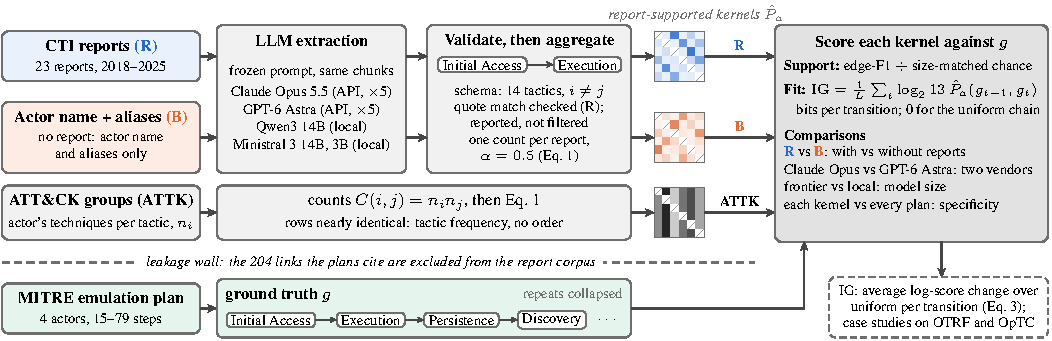
\includegraphics[width=\textwidth]{fig_method}
\caption{Study design. Each row builds one kind of actor kernel (R, B, ATTK) and scores it against the plan's tactic sequence $g$. The dashed line separates the report corpus from the plans that define ground truth. Glyphs are schematic.}
\label{fig:method}
\end{figure*}
Figure~\ref{fig:method} reads left to right, and each row builds one kind of kernel for an actor. \emph{R} is report-conditioned, so a language model reads the actor's reports. \emph{B} is the no-report baseline, in which the model receives only the actor's name and its ATT\&CK v18.1 aliases. It measures performance without the supplied reports; prior knowledge, inference from the actor's name, and, for menuPass, the mismatch between the plan's subgroup and period and those of our reports cannot be separated here. Each no-report generation returns one edge set, used as a binary count matrix in \eqref{eq:est}; we draw five generations per API model and one at temperature 0 per local model and average their scores. Only the schema check applies. The same $\alpha$ does not give every kernel the same smoothing, because row totals differ. A kernel built from one binary edge set can place at most $(1+\alpha)/(1+(K-1)\alpha)=0.20$ on a transition (1.38 bits above uniform). Report kernels built from five to seven reports reach 0.48--0.56 (2.64--2.85 bits), and the ATT\&CK kernel's counts are large enough that smoothing barely affects it. \emph{ATTK} uses no language model. Its counts are $C_a(i,j)=n_i n_j$, where $n_i$ counts the actor's ATT\&CK techniques under tactic $i$ (up to 225). After \eqref{eq:est}, every row for a tactic the actor uses is nearly the same distribution over next tactics (rows for unused tactics are uniform), so ATTK carries tactic frequency but no ordering. The uniform chain, \emph{Uni}, is the null. R and B kernels pass through two steps:
\begin{enumerate}\setlength{\itemsep}{1pt}\setlength{\parskip}{0pt}
\item \textbf{LLM extraction.} Each report is split into chunks of about 6,000 tokens with 300 tokens of overlap, identical for every model. Each chunk is sent with a fixed prompt, asking for the ordered tactic transitions the excerpt states or directly implies, restricted to the 14 tactic names, each with a verbatim evidence passage and a confidence. The prompt forbids adding steps from the model's own knowledge and delimits the excerpt as data.\footnote{Prompts, code, and supplementary tables: \url{https://github.com/jackdmoody/CTI-Transitions}.}
\item \textbf{Validate, then aggregate.} Output must parse as JSON, use only the 14 tactic names, and have $i\neq j$; invalid output gets one retry and is otherwise logged and skipped. After the retry, 40 of 222 calls still failed for Ministral 14B, 8 of 222 for Qwen 14B, 13 of 216 for Ministral 3B, and none for the API models; the local models' retries resend the identical request and so rarely recover, and failed calls contribute no edges. The evidence check (fixed in place before results) splits each evidence span on ellipses, normalizes whitespace, quotes, and dashes, and requires every fragment of at least 8 characters to appear verbatim in the source, in order; spans that fail are \emph{quote-match failures} (we also report a strict whole-span variant). A match confirms that the cited passage exists in the report; it does not verify the tactic labels, the direction, or the adjacency of the extracted transition. The check measures grounding and does not filter, so every schema-valid edge counts once per report however many chunks support it, whether or not its quote matches, giving the counts $C_a$ of \eqref{eq:est}.
\end{enumerate}

\section{Experimental Design}

\paragraph{Actors and ground truth.} Table~\ref{tab:actors} lists the actors. For each plan we take the tactics of its steps in plan order and collapse consecutive repeats. The APT29 plan's two independent scenarios form separate segments; transitions are taken only within a segment, never across the boundary, and the plan's edge set is the union of its segments' edges. The Sandworm plan's Detection and Protection scenarios run the same steps under different security controls, so we use that chain once. The other plans each describe one operation, whose Linux and Windows steps are sequential parts of it rather than alternative executions, so cross-platform handoffs are kept. Each step takes the single tactic the plan assigns to it, including the 26 steps whose technique maps to more than one tactic; the one step whose label is not a tactic takes its technique's first-listed tactic. Neither changes an edge. The menuPass plan marks two steps optional; we include them, and excluding them leaves four edges. Plans, extracted transitions, and telemetry labels share one mapping into the frozen 14-tactic vocabulary. SigmaHQ r2026-07-01 has no Defense Evasion tag, so we map its \texttt{stealth} and \texttt{defense-impairment} tags to Defense Evasion.

\begin{table}[t]
\centering
\small
\begin{tabular}{@{}lllrr@{}}
\toprule
Actor & Nation & Plan source & Steps & GT edges \\
\midrule
APT29 & Russia & ATT\&CK Evals R2 & 79 & 28 \\
OilRig & Iran & CTID & 44 & 15 \\
Sandworm & Russia & CTID & 40 & 21 \\
menuPass & China & CTID & 15 & 6 \\
\bottomrule
\end{tabular}
\caption{Actors and ground truth (distinct edges within scenarios, after collapsing repeats).}
\label{tab:actors}
\end{table}

\paragraph{CTI corpus.} We assembled 23 reports (2018--2025) from government advisories and vendor research, all fetched and hashed. APT29 had seven reports, menuPass five, OilRig five, and Sandworm six. For menuPass, one report covers core APT10 and four cover the MirrorFace/Earth Kasha subgroup that vendors place under the APT10 umbrella.\flag{F6} Two Sandworm documents carry little text (a blog post summarizing a PDF report, and a 492-word landing page); we kept them as fetched rather than substituting fuller sources. We release each report's URL and a hash of its extracted text, not the text itself.

\paragraph{Leakage control.} The CTI used to build an actor's model must be disjoint from the material that defines its ground truth. Every link cited anywhere in a plan or its documentation (204 links across the four plans) is excluded from the report corpus, and a build-time check enforces this after redirect normalization. All but one report (a 2019 APT29 report) postdate the plan they are paired with, so the plans cannot draw on them; one Sandworm report appeared the day after its plan. Exclusion controls which documents we supply, not what a model already knows; the no-report condition measures how the models perform without the supplied documents.

\paragraph{Models.} We compare two frontier models used through their APIs, Claude Opus 5.5 and GPT-6 Astra, with three open-weight models run locally (Qwen3 14B, Ministral 3 14B, and Ministral 3 3B). The API models take no temperature setting, so each extraction runs five times and we report means; local models run at temperature 0, and we also run each 14B model five times at its default sampling. GPT-6 Astra tests whether Claude Opus's no-report results are specific to one vendor.

\paragraph{Metrics.} Each kernel gets three scores. \emph{Edge-F1} is divided by its expected value under random edge sets of the same size, computed exactly from the hypergeometric distribution, as are the percentiles we report against chance. Because the random sets match the prediction's size $k$, this ratio (F1 $\div$ chance) equals precision divided by the base rate $|E_g|/K(K-1)$. It measures precision enrichment, not the precision--recall balance that edge-F1 summarizes, and it is comparable within an actor but not across actors, so we report raw edge-F1 alongside it. \emph{IG} is computed on each plan's transitions (APT29 45, OilRig 17, Sandworm 25, menuPass 6), with 95\% intervals from 10{,}000 resamples of transitions and a block bootstrap (blocks of 2, 3, or 5 transitions kept within a scenario) as a check on dependence. \emph{Specificity} asks which actor's kernel gives each plan the highest likelihood, and also scores each kernel against every plan by edge-F1. To compare performance with and without the supplied reports, each \emph{gap} R$-$B subtracts the no-report kernel's score from the report-conditioned kernel's, for raw edge-F1, F1 $\div$ chance, and IG. A difference in F1 $\div$ chance is a difference in precision scaled by $K(K-1)/|E_g|$. Gap intervals come from 10{,}000 resamples of reports, and we call a gap \emph{clear} only if a leave-one-report-out jackknife interval also excludes zero. The jackknife matters most for IG, whose report-resampled intervals tended to sit below their point estimates in our runs. A resample of $n$ reports keeps on average $n\bigl(1-(1-1/n)^n\bigr)$ distinct reports (3.4 of 5), and Claude Opus's OilRig IG was 0.30, 0.42, 0.53, and 0.62 bits with two to five distinct reports. For grounding, the quote-match failure rate is the share of evidence quotes that fail the check.
\section{Results}

Each paragraph reports Claude Opus, then GPT-6 Astra, then the local models from largest to smallest, and the ATT\&CK kernel last.


\begin{table*}[t]
\centering
\small
\setlength{\tabcolsep}{5pt}
\begin{tabular}{@{}lccccc@{}}
\toprule
 & \multicolumn{5}{c}{Report-conditioned (R)} \\
\cmidrule(l){2-6}
Actor (GT edges) & Claude Opus & GPT-6 Astra & Qwen 14B & Ministral 14B & Ministral 3B \\
\midrule
APT29 (28) & 0.371 (1.99) & 0.450 (2.21) & 0.358 (2.00) & 0.333 (2.03) & 0.133 (0.81) \\
OilRig (15) & 0.396 (3.23) & 0.341 (2.72) & 0.205 (2.02) & 0.375 (3.31) & 0.204 (1.78) \\
Sandworm (21) & 0.372 (2.65) & 0.331 (2.22) & 0.340 (2.44) & 0.167 (1.73) & 0.162 (1.62) \\
menuPass (6) & 0.300 (5.78) & 0.181 (3.30) & 0.270 (4.89) & 0.267 (5.06) & 0.229 (4.18) \\
\midrule
 & \multicolumn{4}{c}{No report (B)} & \\
\cmidrule(lr){2-5}
 & Claude Opus & GPT-6 Astra & Qwen 14B & Ministral 14B & ATT\&CK kernel \\
\midrule
APT29 (28) & 0.234 (1.96) & 0.177 (1.65) & 0.200 (2.17) & 0.100 (1.08) & 0.238 (0.94) \\
OilRig (15) & 0.116 (1.37) & 0.149 (2.37) & 0.071 (0.93) & 0.000 (0.00) & 0.204 (1.38) \\
Sandworm (21) & 0.183 (1.85) & 0.181 (2.45) & 0.118 (1.33) & 0.118 (1.33) & 0.207 (1.00) \\
menuPass (6) & 0.495 (10.87) & 0.323 (8.87) & 0.211 (4.67) & 0.222 (5.06) & 0.069 (1.10) \\
\bottomrule
\end{tabular}
\caption{Support recovery. Edge-F1 against each plan, with F1 $\div$ exact chance in parentheses. API models are means of five runs. Compare ratios within a row.}
\label{tab:recovery}
\end{table*}


\begin{table}[t]
\centering
\small
\setlength{\tabcolsep}{3.5pt}
\begin{tabular}{@{}lccccc@{}}
\toprule
Kernel & APT29 & OilRig & Sandworm & menuPass & Attr. \\
\midrule
\multicolumn{6}{@{}l}{\emph{Report-conditioned (R)}} \\
Claude Opus & $+$.11 & \textbf{$+$.62} & $+$.31 & \textbf{$+$.91} & 3/4 \\
GPT-6 Astra & \textbf{$+$.30} & $+$.55\textsuperscript{*} & $+$.18 & $+$.39\textsuperscript{*} & 3/4 \\
Qwen 14B & $+$.12 & $-$.17\textsuperscript{*} & $+$.17 & \textbf{$+$1.00} & 1/4 \\
\quad sampled & $+$.10 & $-$.21\textsuperscript{*} & $-$.02 & \textbf{$+$.86} & 1/4 \\
Ministral 14B & $+$.16 & \textbf{$+$.37} & $-$.04 & \textbf{$+$1.04} & 3/4 \\
\quad sampled & $+$.13 & $+$.07 & $+$.06 & \textbf{$+$1.07} & 2/4 \\
Ministral 3B & $-$.24\textsuperscript{\dag} & $+$.08 & $+$.01 & \textbf{$+$.89} & 0/4 \\
\multicolumn{6}{@{}l}{\emph{No report (B)}} \\
Claude Opus & $+$.06 & $+$.01 & $-$.02 & \textbf{$+$1.01} & 2/4 \\
GPT-6 Astra & $+$.00 & $+$.05 & $+$.01 & $+$.40\textsuperscript{*} & 2/4 \\
Qwen 14B & $+$.10 & $-$.11 & $-$.07 & $+$.32\textsuperscript{*} & 1/4 \\
Ministral 14B & $-$.01 & $-$.19\textsuperscript{\dag} & $-$.01 & $+$.32\textsuperscript{*} & 1/4 \\
ATT\&CK kernel & $-$.61\textsuperscript{\dag*} & $-$.05 & $-$.30\textsuperscript{\dag} & $-$.92\textsuperscript{*} & 1/4 \\
\bottomrule
\end{tabular}
\caption{Predictive fit. Information gain over the uniform chain on each actor's own plan, in bits per transition. Bold and \dag{} mark 95\% intervals above and below zero, and * a status change under block resampling (see Metrics). Attr.\ counts correct attributions.}
\label{tab:ig}
\end{table}

\paragraph{The frontier kernels match the plans; the ATT\&CK kernel does not.} On edges (Table~\ref{tab:recovery}), Claude Opus's report kernels reach 2.0--5.8 times chance, at or above the 99.7th percentile for every actor, and GPT-6 Astra's reach 2.2--3.3 times, at or above the 97th. Both 14B models exceed chance for every actor, though Qwen 14B on OilRig (93rd percentile) and Ministral 14B on Sandworm (84th) fall short of the 95th; Ministral 3B falls below chance on APT29. In likelihood (Table~\ref{tab:ig}), Claude Opus's and GPT-6 Astra's chains beat the uniform chain on all four plans, clearly on two for Claude Opus (OilRig and menuPass) and on one for GPT-6 Astra (APT29; its OilRig interval, $[-0.01, 1.08]$, includes zero); Ministral 14B's beat it on three, Qwen 14B's clearly only on menuPass, and Ministral 3B's clearly only on menuPass while falling clearly below uniform on APT29. The ATT\&CK kernel, which knows every tactic the actor uses but not their order, sits at chance on edges (0.94--1.38 times; for Sandworm its edge set is all 182 edges) and below uniform on every plan, clearly so for Sandworm and, under i.i.d.\ resampling, APT29. The frontier kernels therefore outperform the tested ATT\&CK frequency baseline on these plans; because that baseline differs from them in both its evidence and its count scale, the comparison does not isolate the value of ordering.

\begin{table}[t]
\centering
\small
\begin{tabular}{@{}lcccc@{}}
\toprule
Kernel $\backslash$ plan & APT29 & OilRig & Sandworm & menuPass \\
\midrule
APT29 & \textbf{.371} & .286 & .252 & .183 \\
OilRig & .341 & \textbf{.396} & .328 & .145 \\
Sandworm & .296 & .285 & \textbf{.372} & .052 \\
menuPass & .400 & .367 & .288 & \textbf{.300} \\
\bottomrule
\end{tabular}
\caption{Specificity. Edge-F1 of each Claude Opus report kernel (rows) against each plan (columns). Descriptive only, since a row's maximum depends on plan size.}
\label{tab:h4}
\end{table}

\paragraph{Specificity is partial.} On each fixed plan, we ask which actor's kernel gives it the highest likelihood (Table~\ref{tab:ig}, Attr.). Claude Opus, GPT-6 Astra, and Ministral 14B attribute 3 of 4 plans correctly, Qwen 14B 1, and Ministral 3B none; no-report kernels manage at most 2, and both frontier models confuse APT29 and menuPass. Edge overlap with each plan held fixed agrees (Claude Opus 3 of 4, GPT-6 Astra 4, Qwen 14B and Ministral 14B 3 each, Ministral 3B none). Table~\ref{tab:h4} shows the full overlap matrix for Claude Opus; we treat it as descriptive, because a row's maximum depends on the sizes of the plans it is compared against. These are results for four plans, not for independent campaigns.


\begin{table*}[t]
\centering
\small
\setlength{\tabcolsep}{4pt}
\begin{tabular}{@{}lrcccccc@{}}
\toprule
 & & \multicolumn{3}{c}{Claude Opus} & \multicolumn{3}{c}{GPT-6 Astra} \\
\cmidrule(lr){3-5}\cmidrule(l){6-8}
Actor & Refs. & $\Delta$F1 & $\Delta$enrichment & $\Delta$IG & $\Delta$F1 & $\Delta$enrichment & $\Delta$IG \\
\midrule
APT29 & 44 & $+$0.137 & $+$0.03 & $+$0.06 & \textbf{$+$0.273} & $+$0.56 & $+$0.30 \\
 & & {\scriptsize [$-$0.098, $+$0.177]} & {\scriptsize [$-$0.85, $+$0.44]} & {\scriptsize [$-$0.27, $+$0.11]} & {\scriptsize [$+$0.023, $+$0.342]} & {\scriptsize [$-$0.41, $+$1.33]} & {\scriptsize [$-$0.19, $+$0.40]} \\
OilRig & 28 & \textbf{$+$0.280} & \textbf{$+$1.86} & \textbf{$+$0.61} & \textbf{$+$0.193} & $+$0.34 & \textbf{$+$0.50} \\
 & & {\scriptsize [$+$0.185, $+$0.329]} & {\scriptsize [$+$1.29, $+$2.98]} & {\scriptsize [$+$0.07, $+$0.69]} & {\scriptsize [$+$0.115, $+$0.297]} & {\scriptsize [$-$0.56, $+$2.16]} & {\scriptsize [$+$0.02, $+$0.66]} \\
Sandworm & 26 & $+$0.189 & $+$0.80 & $+$0.33 & $+$0.150 & $-$0.22 & $+$0.17 \\
 & & {\scriptsize [$-$0.012, $+$0.255]} & {\scriptsize [$-$0.05, $+$1.79]} & {\scriptsize [$-$0.11, $+$0.46]} & {\scriptsize [$-$0.092, $+$0.217]} & {\scriptsize [$-$1.69, $+$0.64]} & {\scriptsize [$-$0.25, $+$0.32]} \\
menuPass & 20 & $-$0.195 & $-$5.08 & $-$0.09 & \textbf{$-$0.143} & \textbf{$-$5.57} & $-$0.01 \\
 & & {\scriptsize [$-$0.491, $-$0.062]} & {\scriptsize [$-$10.73, $-$1.52]} & {\scriptsize [$-$1.22, $+$0.37]} & {\scriptsize [$-$0.307, $-$0.082]} & {\scriptsize [$-$8.85, $-$3.47]} & {\scriptsize [$-$0.68, $+$0.20]} \\
\bottomrule
\end{tabular}
\caption{R $-$ B for the frontier models in raw edge-F1, F1 $\div$ exact chance, and IG (bits per transition), with 95\% intervals from 10{,}000 resamples of reports. Bold marks a clear gap, whose jackknife interval also excludes zero. Refs.\ counts ATT\&CK group-page references.}
\label{tab:h2}
\end{table*}

\paragraph{With and without the supplied reports, the answer depends on actor and metric.} We expected report-conditioned kernels to beat no-report kernels on edge precision, recall, and F1 for each actor and model, and the gap to grow as public coverage shrinks. Neither expectation held. Table~\ref{tab:h2} shows three patterns. First, on raw edge-F1 the reports usually help, with the report-conditioned kernel scoring higher for every actor except menuPass under Claude Opus and GPT-6 Astra, and for every actor under both 14B models. The gain is clear for OilRig under Claude Opus, GPT-6 Astra, and Ministral 14B, and for APT29 under GPT-6 Astra. Report kernels also list more edges (1.2--3.3 times as many; 3.6--5.4 times for GPT-6 Astra). Second, once the chance control turns the comparison into one of precision, the reports clearly help only for OilRig under Claude Opus, Sandworm under Qwen 14B, and OilRig under Ministral 14B, and for no actor under GPT-6 Astra. Every APT29 enrichment interval spans zero. Third, menuPass reverses for both frontier models. GPT-6 Astra's gap is clear (jackknife $[-6.87, -4.26]$), and Claude Opus's is negative whichever report is left out ($-7.21$ to $-3.47$), although its jackknife interval reaches zero. Without the reports, Claude Opus recalls on average 80\% of the plan's six edges with about 13 predicted edges. Neither 14B model shows a clear reversal. The coverage expectation fails for every model. Rank correlations between the gap and shrinking coverage, expected to be positive, are $-0.4$ for Claude Opus, $-1.0$ for GPT-6 Astra, $+0.4$ for Qwen 14B (whose OilRig and Sandworm gaps are nearly equal), and $-0.8$ for Ministral 14B. Ministral 3B is not interpretable because, without a report, it returned an empty list in 19 of 24 calls, the answer the prompt asks for when a model knows nothing reliable about the actor.

In likelihood, the reports help only on OilRig. With intervals from resampling reports (Table~\ref{tab:h2}), the advantage is clear for Claude Opus ($+0.61$ bits per transition [0.07, 0.69]), GPT-6 Astra ($+0.50$ [0.02, 0.66]), and Ministral 14B ($+0.56$ [0.16, 0.64]). Only Claude Opus's holds up under two further checks. GPT-6 Astra's does not exclude zero when the plan's transitions are resampled instead ($[-0.02, 1.00]$), and Ministral 14B's does not survive removing edges whose quotes fail. On menuPass, neither frontier model's likelihood difference excludes zero ($-0.09$ and $-0.01$), so the no-report outputs have higher edge-F1 and enrichment without an established likelihood advantage.

\paragraph{Small open models recover structure, not grounding.} We expected a 14B open model to reach at least 80\% of Claude Opus's edge-F1. At temperature 0, Qwen 14B reaches 96\%, 52\%, 91\%, and 90\% of it for APT29, OilRig, Sandworm, and menuPass, and Ministral 14B 90\%, 95\%, 45\%, and 89\%, so each meets the criterion for three of four actors, but not the same three; Ministral 3B meets it for none (36--76\%). Sampled runs are weaker for Qwen 14B, which occasionally loops (up to 115 transitions from one chunk), and mixed for Ministral 14B. The larger gap is grounding. The quote-match failure rate is at most .005 for Claude Opus and zero for GPT-6 Astra, but .07--.29 by actor for Qwen 14B, .20--.30 for Ministral 14B, and .50--.68 for Ministral 3B, and Ministral 14B also failed the output schema on 40 of 222 calls, none of which the retry recovered, so those calls contribute nothing to its kernels. Removing edges whose quotes fail leaves the frontier kernels essentially unchanged and the 14B models' structure result intact (same three actors), but Qwen 14B's Sandworm gap and Ministral 14B's OilRig likelihood advantage are no longer clear, and attribution improves for Qwen 14B and Ministral 3B. On an air-gapped network, where only such models can run, every extracted transition therefore needs a mechanical check against its source. The local models refused nothing and ran at 41--57\,s per call for the 14B models; Claude Opus refused 11 of 185 calls, including every sample of the OpTC red-team ground-truth document.

\section{Case Study: Using CTI for Hunting on Public Telemetry}

We expected conditioning on CTI to improve hunting, tested by injecting each actor's chain, at the tactic level, into benign host telemetry and comparing CTI-conditioned with unconditioned scoring. This needs a tactic mapper; we built one from SigmaHQ's Windows rules \citep{sigmahq} (release r2026-07-01; 2,017 rules), excluded 56 actor- or malware-specific rules, and froze it before any scoring. None of the public corpora we screened passed the go/no-go thresholds we set before scoring. On OpTC, a mapper restricted to rules evaluable on both eCAR and Sysmon (707 of 3,174 queries) tags $3\times10^{-6}$ of benign events, in one tactic, and leaves the injected chains 27, 3, 1, and 3 visible transitions per actor; adding SigmaHQ's threat-hunting rules raises the benign tag rate only to $2.4\times10^{-5}$, against thresholds of at least four benign tactics, a benign tag rate of at least $10^{-4}$, and at least ten visible transitions per actor. We therefore turn to two recorded executions, an APT29 emulation and a red-team operation.

\paragraph{Case study A: a recorded APT29 emulation.} On the OTRF recording of the APT29 emulation, the frozen mapper recovers 8 tactics and 37 transitions, with no Discovery, Command and Control, Exfiltration, or Initial Access, and matches the plan at 2.07$\times$ chance. Support recovery shows little actor specificity. Claude Opus's APT29 kernel reaches 1.45$\times$ chance, no better than its OilRig kernel, although GPT-6 Astra's (1.79$\times$) beats its other actors' kernels (1.08--1.63$\times$). For likelihood, the plan-level result inverts. Among the APT29 kernels, only the ATT\&CK kernel is clearly above uniform ($+0.76$ bits per transition, 95\% interval $[0.50, 0.98]$), while the extracted APT29 chains sit at or below zero (Claude Opus $-0.12$ $[-0.34, 0.10]$, GPT-6 Astra $-0.04$ $[-0.28, 0.19]$). The OilRig and menuPass ATT\&CK kernels are also clearly above uniform, so the gain is not actor-specific. The basis, 37 transitions from one recording, is thin.

\paragraph{Case study B: a red-team execution on OpTC.} OpTC's red team emulated no named APT, so every actor kernel is off-target. With corrected labels \citep{majorczyk2025optc}, 235,698 events on the 29 red-team hosts are malicious and the mapper tags 160 of them (0.07\%); the test set has 4,428 windows of eight tagged events, 46 positive. At first, the pipeline scored uncollapsed windows with a self-transition cell in each row, which lets the ATT\&CK kernel lead (AUPRC .19--.37) through generic Defense Evasion repetition that a kernel built from all ATT\&CK groups matches (.306). Scored as the model defines, the frontier models' report kernels reach .28--.43 (Claude Opus) and .18--.47 (GPT-6 Astra) against .18 for uniform. That gain is neither actor-specific nor robust. None of these kernels describes this red team; oracle kernels compiled from the red team's own ground truth by GPT-6 Astra and the local models stay at uniform (Claude Opus refused the document). Claude Opus's gain survives dropping the five hosts that run one scripted benign job, 91\% of negative windows (.38--.68 against .19; 29 positive windows remain), but vanishes when only that job's two rules are removed (.15--.19 against .15; 45 remain). Equation~\eqref{eq:diff} shows where the room for gains is limited. Of the 46 positive windows, 11 contain no tactic change and so receive no contribution from any actor kernel, and 7 contain one, although a single informative transition can still raise a window's score.

\section{Discussion}

\paragraph{The plan and the sensor.} Extracted kernels predict the emulation plans better than the tested ATT\&CK frequency baseline does; because that baseline differs in both its evidence and its count scale, this does not by itself isolate the value of ordering. On the recorded APT29 run, as seen through the mapper, the two swap places, and only the ATT\&CK frequency kernels beat uniform. One explanation is that a rule-based mapper reports the tactics its rules fire on most, which favors a frequency model over a sequence model. CTI describes the operation and the mapper describes the sensor, so a hunting evaluation must measure both.

\paragraph{Document control is not knowledge control.} Our leakage rule excluded every source the plans cite, yet for menuPass both frontier models' no-report outputs had higher edge-F1 and enrichment than their report-conditioned kernels, without an established likelihood advantage, and this holds when the plan's two optional steps are removed. The no-report condition cannot say why. The plan reflects older APT10 reporting that the models may have seen,\flag{F7} our reports describe a newer subgroup, and a model can also infer plausible transitions from an actor's name. Emulation-plan ground truth can therefore reward knowledge of the very sources a study excludes. Neither 14B model shows the reversal, which fits a role for prior knowledge but does not prove it.

\paragraph{A checklist for evaluating LLM-compiled CTI.} Each control below changed or qualified one of our conclusions; parentheses point to the evidence.
\begin{itemize}
\item Report a no-report baseline beside every report-conditioned result, even after excluding every source the ground truth cites, and state each claim per metric (menuPass, Table~\ref{tab:h2}).
\item Score with a proper scoring rule such as IG, and control edge-F1 for the number of predicted edges; the size-matched ratio measures precision, not precision--recall balance (Tables~\ref{tab:ig} and~\ref{tab:h2}).
\item Resample both reports and plan transitions, keep blocks within scenarios, and check that a result survives leaving out each report in turn (Tables~\ref{tab:ig} and~\ref{tab:h2}).
\item Check every evidence quote mechanically against its source, report the failure rate per model (7--30\% for the 14B models), and show what removing failed-quote edges changes; a match shows that a passage exists, not that it supports the transition.
\item Use the uniform chain as the detection null and score windows as the model defines them (case B, as first run versus as defined).
\item Measure how much behavior the telemetry exposes before testing detection (go/no-go; Eq.~\eqref{eq:diff}).
\item Characterize the benign side of a hunting test set (on OpTC, one scripted job supplied 91\% of the negative windows).
\end{itemize}

\paragraph{Future work.} Each finding points to a next study. \emph{Separating the reports' contribution from prior knowledge:} counterfactual reports, in which the order of two described steps is swapped or the actor is renamed, would show directly whether a chain follows the text or the model's prior knowledge. Plans for intrusions reported after a model's training cutoff would remove prior knowledge as an explanation, provided the cutoff is measured rather than taken from documentation, since effective cutoffs often differ from reported ones \citep{cheng2024dated}. \emph{Grounding small models:} extraction that returns character offsets instead of quotes guarantees that every cited passage exists, leaving only whether it supports the transition, which a decompose-then-verify check could test \citep{wanner2025dndscore}; and because the two 14B models fail on different actors, combining them may cover what each misses. \emph{Observation:} a hidden Markov model with tactics as hidden states, the mapper as a noisy emission model, and compiled chains as actor priors would let a detector reason about tactics it cannot see directly, as monitoring of Bayesian attack graphs does for hidden attack progress \citep{kazeminajafabadi2023monitoring}, and the same priors could guide which hosts or sensors to watch. Telemetry beyond process creation would give such a detector more to see; a quarter of OpTC's attack windows contain no tactic change at all. \emph{Sharper actor models:} a hierarchical prior that shrinks each actor toward a population chain rather than toward uniform, more independent reports per actor, and extraction of each report's ordered path rather than its set of transitions would raise the ceiling of Eq.~\eqref{eq:diff} and let counts track how often an actor makes a transition rather than how often reports mention it. \emph{Richer dynamics:} higher-order and semi-Markov chains would keep the context and dwell times we discard, and mixtures over subgroups would fit actors like menuPass better than one stationary chain. More actors, technique-level ground truth, and incident-response timelines in place of emulation plans would make each of these testable.

\section{Limitations}

Ground truth is small (menuPass's plan yields six edges), and with four actors, cross-actor patterns are descriptive. Emulation plans are curated reconstructions, not intrusion records; menuPass kernels draw on an APT10-umbrella subgroup, and two Sandworm documents are thin. Behavior is modeled as the first-order embedded jump chain over collapsed tactics, and this structure is assumed rather than tested. Extraction returns a set of transitions per report rather than an ordered path, so the data cannot distinguish a first-order chain from higher-order or non-Markov dynamics. As noted beside Eq.~\eqref{eq:est}, extracted transitions record described precedence rather than one-step adjacency. The estimator counts report-level support rather than observed transitions, so it measures how often reports describe a transition rather than how often the actor makes it, and its concentration, and hence the bound in Eq.~\eqref{eq:diff}, grows with the number of reports rather than with the number of transitions they describe. Information-gain intervals treat plan transitions as independent; a block bootstrap that keeps blocks within scenarios changes the status of nine cells (Table~\ref{tab:ig}, *). Three sensitivity analyses move individual cells but leave the main conclusions in place. They remove failed-quote edges (local models), cut cross-platform handoffs (mainly OilRig), and drop menuPass's two optional steps, which leaves its plan four edges and lowers both 14B models to two of four actors on the 80\% criterion while leaving the menuPass reversal intact. We also did not grade the reports themselves. A vague or incomplete report limits what any model can extract, and the leave-one-report-out jackknife guards against one weak report but not against a corpus that is weak throughout. Hunting evidence rests on two case studies with thin bases, one dominated by a scripted benign job.

\section{Conclusion}
Language models can compile threat-intelligence prose into report-supported predictive kernels over ATT\&CK tactics. For two frontier models from different vendors, these kernels outperform the tested ATT\&CK frequency baseline on four emulation plans in both edge precision and likelihood. Whether the supplied reports add to what a model produces without them depends on actor and metric. For menuPass, both frontier models' no-report outputs have higher edge-F1 and precision enrichment, without an established likelihood advantage. Evaluations of compiled CTI therefore need no-report baselines, metric-specific claims, proper scoring rules, and report-level uncertainty. Two 14B local models recover much of the structure, though not for the same actors, but need mechanical quote checking; a 3B model does not suffice. Treating compiled intelligence as a Markov chain also makes one limit explicit. Relative to the uniform chain, a kernel can raise a window's score only through its departure from uniform on the transitions the telemetry exposes, and whether that improves detection also depends on benign-window scores. In two case studies on recorded emulation and red-team executions, no robust actor-specific detection benefit was established. Testing that end-to-end will need telemetry, or an observation model, that exposes more of an intrusion than a rule-based tactic mapper does on public data.


\bibliography{references}


\end{document}
